% POAMG Structure Figure
% Compile this file with pdflatex --shell-escape poamg-structure.tex
\documentclass{standalone}
\usepackage{tikz}
\usepackage{amsmath} % For \boldsymbol
\usetikzlibrary{arrows.meta, positioning, shapes, calc, backgrounds, shadows.blur, fit}
\begin{document}
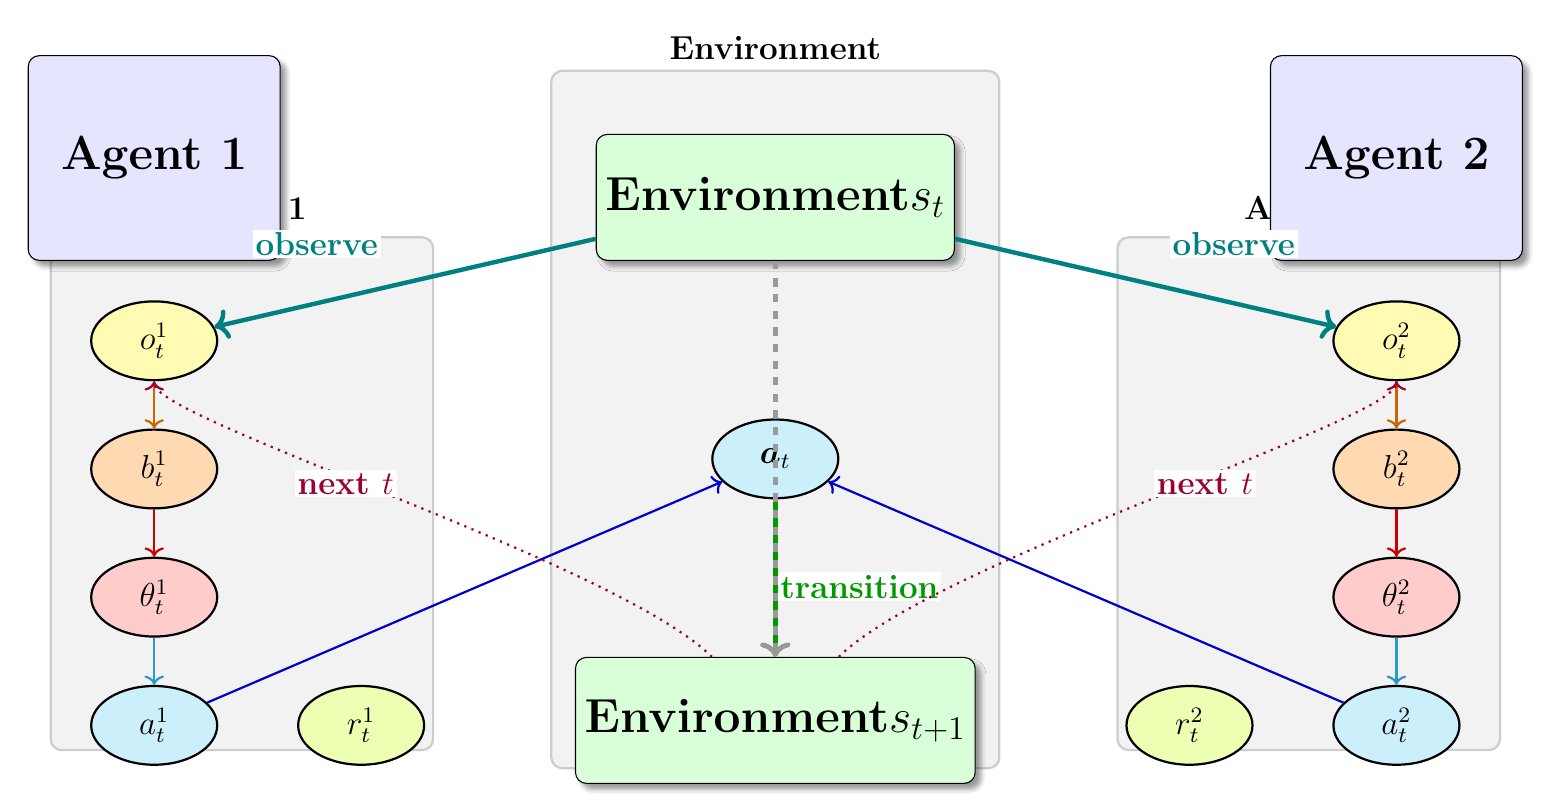
\begin{tikzpicture}[
  agent/.style={draw, rounded corners, fill=blue!10, minimum width=3.2cm, minimum height=2.6cm, font=\LARGE, blur shadow},
  env/.style={draw, rounded corners, fill=green!15, minimum width=3.2cm, minimum height=1.6cm, font=\LARGE, blur shadow},
  obs/.style={draw, fill=yellow!30, ellipse, minimum width=1.6cm, minimum height=1.0cm, font=\large, thick},
  belief/.style={draw, fill=orange!30, ellipse, minimum width=1.6cm, minimum height=1.0cm, font=\large, thick},
  param/.style={draw, fill=red!20, ellipse, minimum width=1.6cm, minimum height=1.0cm, font=\large, thick},
  action/.style={draw, fill=cyan!20, ellipse, minimum width=1.6cm, minimum height=1.0cm, font=\large, thick},
  reward/.style={draw, fill=lime!30, ellipse, minimum width=1.6cm, minimum height=1.0cm, font=\large, thick},
  groupbox/.style={fill=gray!10, rounded corners, draw=gray!40, thick, inner sep=0.3cm},
  legendbox/.style={fill=white, draw=black, rounded corners, thick, inner sep=0.2cm},
  every node/.style={font=\large}
]
% Environment state
\node[env] (env) at (0,0) {\textbf{Environment}\\$s_t$};

% Agents
\node[agent, left=4.0cm of env, yshift=0.5cm] (agent1) {\textbf{Agent 1}};
\node[agent, right=4.0cm of env, yshift=0.5cm] (agent2) {\textbf{Agent 2}};

% Observations
\node[obs, below=0.5cm of agent1] (obs1) {$o^1_t$};
\node[obs, below=0.5cm of agent2] (obs2) {$o^2_t$};

% Beliefs
\node[belief, below=0.6cm of obs1] (belief1) {$b^1_t$};
\node[belief, below=0.6cm of obs2] (belief2) {$b^2_t$};

% Policy params
\node[param, below=0.6cm of belief1] (theta1) {$\theta^1_t$};
\node[param, below=0.6cm of belief2] (theta2) {$\theta^2_t$};

% Actions
\node[action, below=0.6cm of theta1] (action1) {$a^1_t$};
\node[action, below=0.6cm of theta2] (action2) {$a^2_t$};

% Joint action
\node[action, below=2.0cm of env] (jointaction) {$\boldsymbol{a}_t$};

% Next environment state
\node[env, below=2.0cm of jointaction] (envnext) {\textbf{Environment}\\$s_{t+1}$};

% Rewards
\node[reward, right=1.0cm of action1] (reward1) {$r^1_t$};
\node[reward, left=1.0cm of action2] (reward2) {$r^2_t$};

% Arrows: Environment to observations
\draw[->, ultra thick, teal] (env) -- node[above left, xshift=-8pt, yshift=8pt, fill=white, inner sep=1pt] {\textbf{observe}} (obs1);
\draw[->, ultra thick, teal] (env) -- node[above right, xshift=8pt, yshift=8pt, fill=white, inner sep=1pt] {\textbf{observe}} (obs2);

% Observations to beliefs
\draw[->, thick, orange!80!black] (obs1) -- (belief1);
\draw[->, thick, orange!80!black] (obs2) -- (belief2);

% Beliefs to policy params
\draw[->, thick, red!80!black] (belief1) -- (theta1);
\draw[->, thick, red!80!black] (belief2) -- (theta2);

% Policy params to actions
\draw[->, thick, cyan!80!black] (theta1) -- (action1);
\draw[->, thick, cyan!80!black] (theta2) -- (action2);

% Actions to joint action
\draw[->, thick, blue!80!black] (action1) -- (jointaction);
\draw[->, thick, blue!80!black] (action2) -- (jointaction);

% Joint action to environment
\draw[->, ultra thick, green!60!black] (jointaction) .. controls +(0,-1.2) and +(0,1.2) .. node[right, fill=white, inner sep=1pt] {\textbf{transition}} (envnext);

% Environment transition (dashed, for clarity)
\draw[->, ultra thick, dashed, gray!80] (env) .. controls +(0,-1.2) and +(0,1.2) .. (envnext);

% Feedback: Next env to next obs (curved, dotted)
\draw[->, thick, dotted, purple!80!black] (envnext) .. controls +(-2.0,2.0) and +(0,-1.0) .. node[above left, fill=white, inner sep=1pt] {\textbf{next $t$}} (obs1);
\draw[->, thick, dotted, purple!80!black] (envnext) .. controls +(2.0,2.0) and +(0,-1.0) .. node[above right, fill=white, inner sep=1pt] {\textbf{next $t$}} (obs2);

% Background boxes for agents and environment
\begin{pgfonlayer}{background}
  \node[groupbox, fit=(obs1) (belief1) (theta1) (action1) (reward1), label=above:{\textbf{Agent 1}}, yshift=0.5cm, xshift=-0.2cm] (agent1bg) {};
  \node[groupbox, fit=(obs2) (belief2) (theta2) (action2) (reward2), label=above:{\textbf{Agent 2}}, yshift=0.5cm, xshift=0.2cm] (agent2bg) {};
  \node[groupbox, fit=(env) (envnext) (jointaction), label=above:{\textbf{Environment}}, yshift=0.5cm] (envbg) {};
\end{pgfonlayer}

\end{tikzpicture}
\end{document} 